%
% Another appendix chapter
\chapter{Theoretic Limits on Capture}



\section{Unconstrained Capture Region}
\begin{equation}
    x_{balistic}=\sqrt{2}x_{cp}
    \end{equation}

\cite{koolen2016balance}
\begin{figure}[h]
\centering
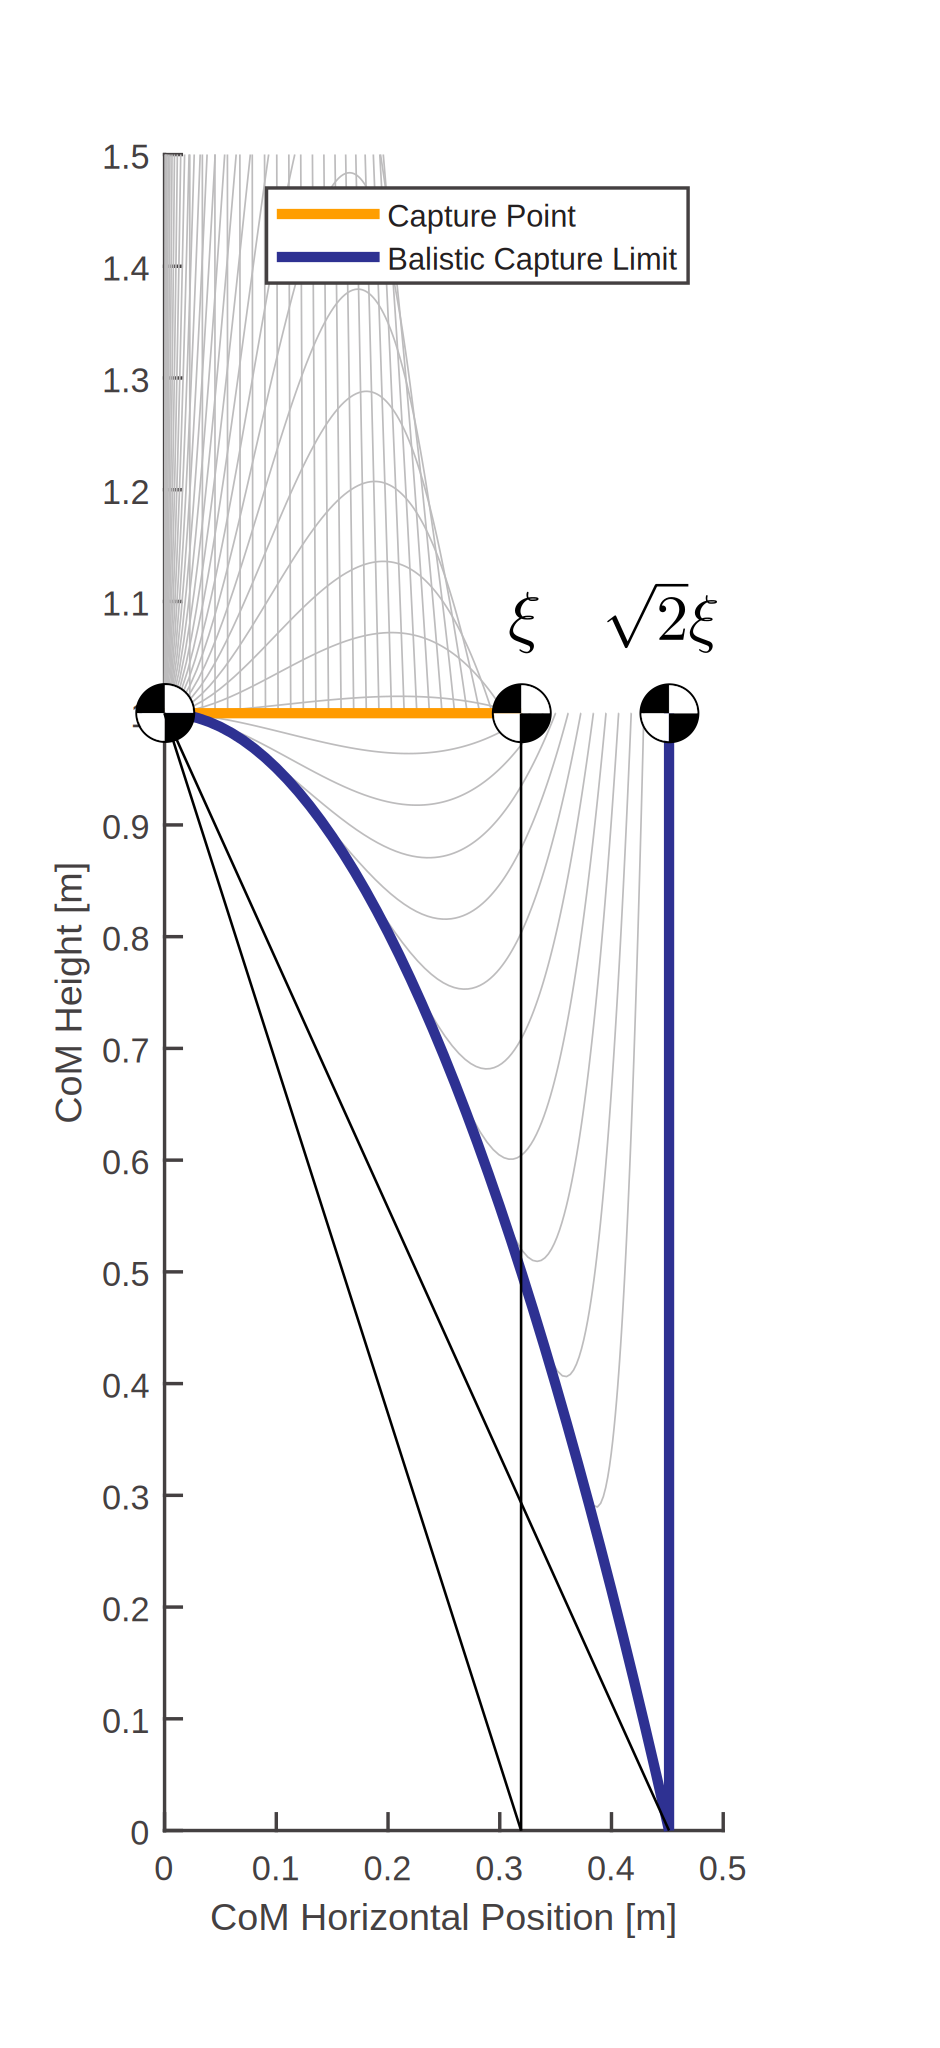
\includegraphics[width=0.3\textwidth]{STYLESTUFF/CPvsBalistic.png}
\caption{}
\label{fig:cpbal}
\end{figure}
\section{Height Constrained Capture}
\begin{equation}
    x_{cp,height}=(\frac{\sqrt{2g\delta z_{max}}}{g}+\sqrt{\frac{z_o+\delta z_{max}}{g}})(\dot{x}_0-\frac{x_0}{z_0}\sqrt{2g\delta z_{max}}).
\end{equation}
\begin{figure}[h]
\centering
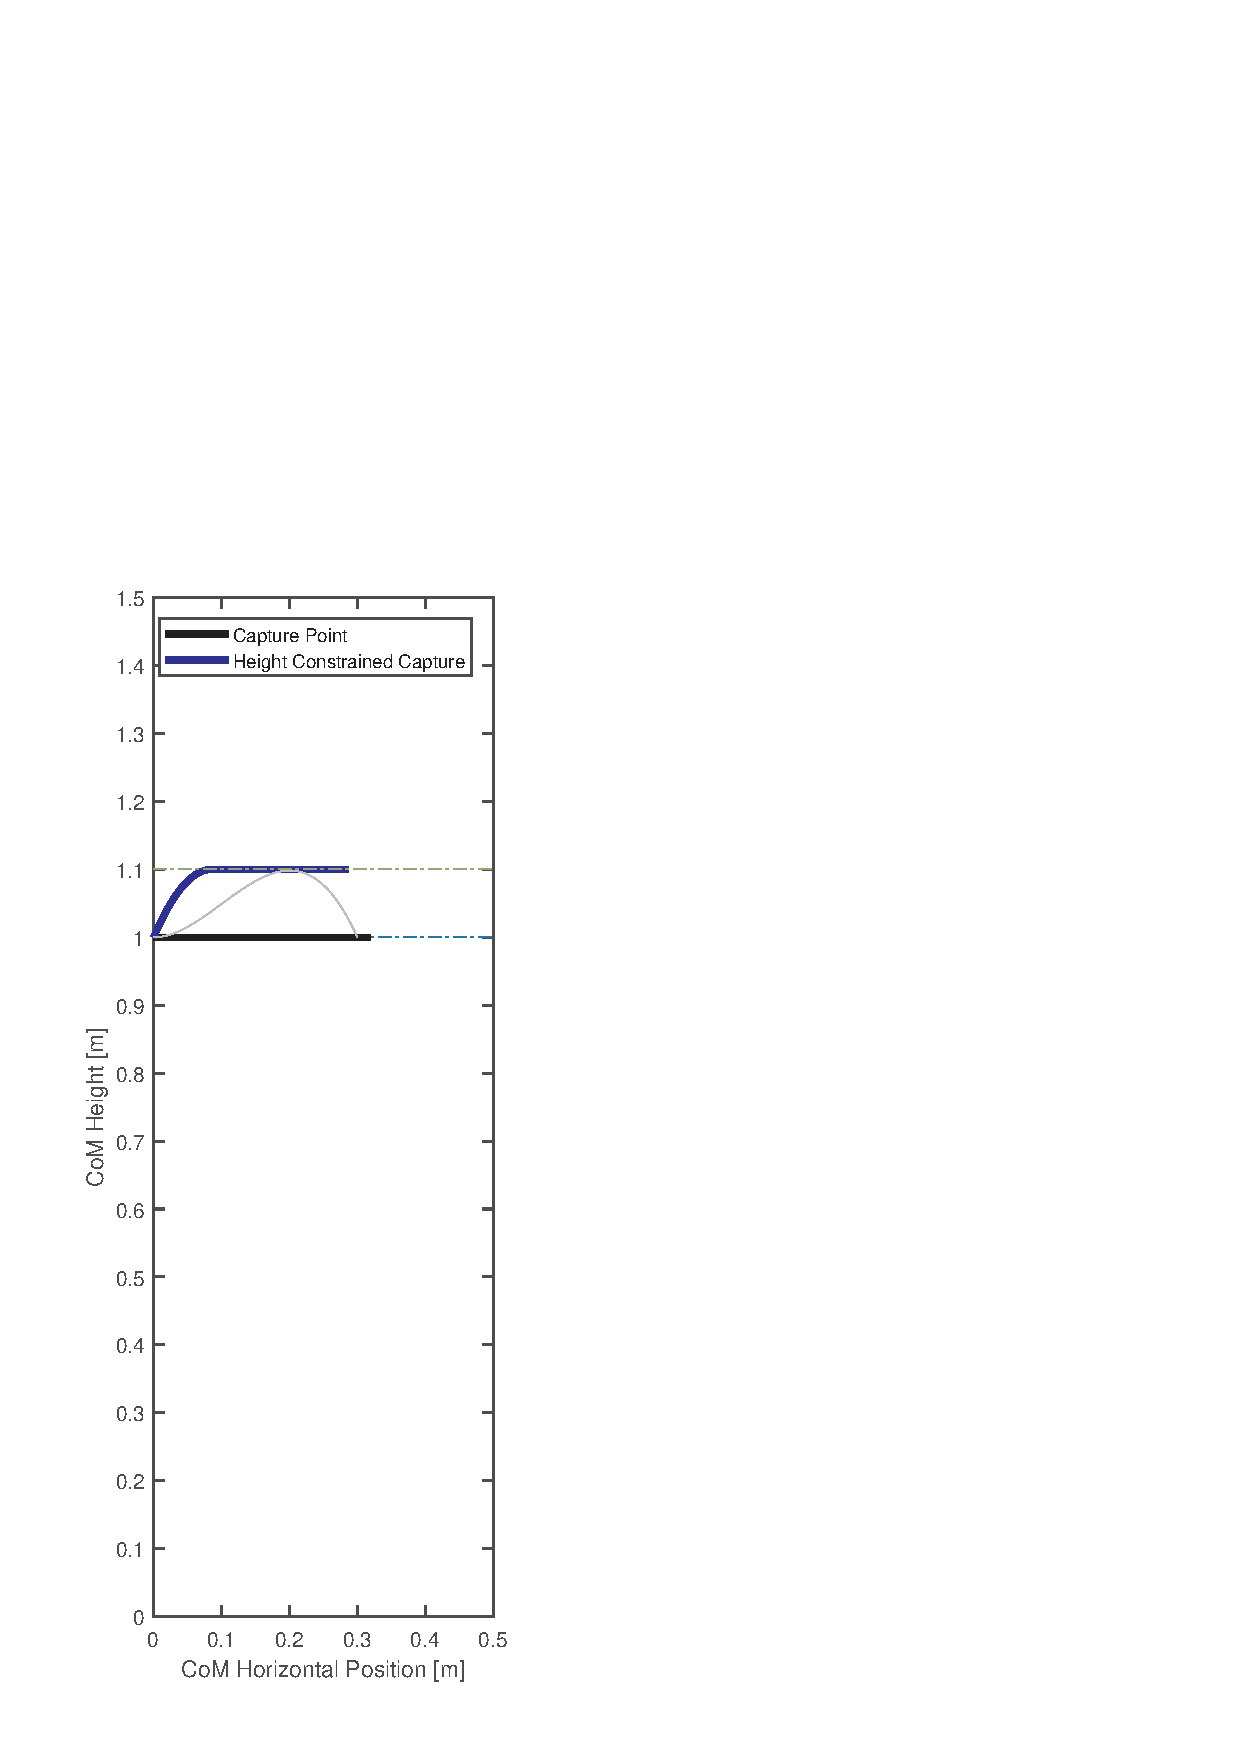
\includegraphics[width=0.3\textwidth]{STYLESTUFF/CPvsHeight.png}
\caption{}
\label{fig:cpbal}
\end{figure}

\section{Impact Influenced Capture}
\cite{kuo2005energetic}